
%Revision Date:  06-20-2021
\chapterimage{Water1.png} % Chapter heading image

\chapter{Introduction to Wastewater Treatment}

% \section{Paragraphs of Text}\index{Paragraphs of Text}


% \everymath{\displaystyle}
% \linespread{2}%controls the spacing between lines. Bigger fractions means crowded lines%
% %\pagestyle{fancy}
% %\usepackage[margin=1 in, top=1in, includefoot]{geometry}
% %\everymath{\displaystyle}
% \linespread{2}%controls the spacing between lines. Bigger fractions means crowded lines%
% %\pagestyle{fancy}
% \pagestyle{fancy}
% \setlength{\headheight}{56.2pt}
% \colorlet{Mycolor1}{green!10!orange!90!}

% \chead{\ifthenelse{\value{page}=1}{
\includegraphics[scale=0.3]{SCC}\\ \textbf \textbf Introduction to Wastewater Treatment}}
% \rhead{\ifthenelse{\value{page}=1}{}{}}
% \lhead{\ifthenelse{\value{page}=1}{}{\textbf Introduction to Wastewater Treatment}}
% \rfoot{\ifthenelse{\value{page}=1}{Module 1: WATR 048 - Spring 2019}{Module 1: WATR 048 - Spring 2019}}

% \cfoot{Page \thepage\ of \pageref{LastPage}}
% \lfoot{Shabbir Basrai}
% \renewcommand{\headrulewidth}{2pt}
% \renewcommand{\footrulewidth}{1pt}

% \newcommand{\stkout}[1]{\ifmmode\text{\sout{\ensuremath{#1}}}\else\sout{#1}\fi}
% %Defining colour with different models.
% \definecolor{mypink1}{rgb}{0.858, 0.188, 0.478}
% \definecolor{mypink2}{RGB}{219, 48, 122}
% \definecolor{mypink3}{cmyk}{0, 0.7808, 0.4429, 0.1412}
% \definecolor{mygray}{gray}{0.6}
% \colorlet{LightRubineRed}{RubineRed!70!}
% \colorlet{Mycolor1}{green!10!orange!90!}
% \definecolor{Mycolor2}{HTML}{00F9DE}

% %New command used in the table with all available colour names
% \newcommand{\thiscolor}[1]{\texttt{#1} \hfill \fcolorbox{black}{#1}{\hspace{2mm}}}

% %This changes the row separation in the table
% \renewcommand{\arraystretch}{1.5}




%\noindent\textsc{Area \& Volume Math Problems}
%\definecolor{shadecolor}{RGB}{200,200,240}
% \item \noindent\textsc{Why Treat Wastewater}
\section{Why Treat Wastewater}\index{Why Treat Wastewater}
\begin{itemize}
\item Wastewater is used water from home and industries\\
\item Wastewater must be treated prior to returning it back into the environment - typically into the receiving waters which include lakes, rivers and ocean.


\item Wastewater treatment removes:
\begin{itemize}
\item organic matter
\item inorganic  pollutants including plant nutrients - nitrogen and phosphorous\\
\item pathogenic (disease causing) organisms\\
\end{itemize}

\item Wastewater treatment protects:
\begin{itemize}
\item The environment
\item Human health
\end{itemize}

\item In the receiving waters, inadequately treated wastewater discharge depletes dissolved oxygen levels - \hl{Eutrophication}, potentially destructing its normal aquatic life including fish.  Wastewater discharge promotes eutrophication due to:

\begin{itemize}
\item Nutrients such as nitrogen and phosphorous present in wastewater effluent promotes growth of plant and algal matter.  Dissolved oxygen is consumed as a part of the normal decay of this plant and algal matter.  
\item The consumption of organic material present in wastewater discharge by aerobic bacteria also results in oxygen depletion in the receiving waters.  


\end{itemize}
\end{itemize}

\section{Wastewater Treatment Regulations}\index{Wastewater Treatment Regulations}
% \begin{snugshade*}
% \item \noindent\textsc{Wastewater Treatment Regulations}
% \end{snugshade*}

\begin{itemize}
\item The \hl{National Pollutant Discharge Elimination System (NPDES) permit program} was created in 1972 by the Clean Water Act (CWA)
\item Applies to sources that discharge pollutants to waters of the United States.
\item Requires all facilities discharging “pollutants” into any body of water in the USA to obtain and comply with a \hl{NPDES permit}
\item NPDES permit \hl{establishes} \textul{discharge limits}, \textul{monitoring} and \textul{reporting} \hl{requirements}\\
\item The NPDES permitting and enforcement responsibilities have been delegated by the EPA to the State of California for implementation through the \hl{State Water Resources Control Board(SWRCB)} and the \textul{nine} \hl{Regional Water Quality Control Boards (Regional Water Boards)}.
\item In California, NPDES permits are also referred to as waste discharge requirements (WDRs) that regulate discharges to waters of the United States.
\end{itemize}


\section{Wastewater Process Overview}\index{Wastewater Process Overview}
Wastewater treatment involves the following elements:

\subsection{Generation}\index{Generation}

Wastewater originates from domestic, industrial, commercial or agricultural activities. The characteristics of wastewater vary depending on the source. Types of wastewater include: 
\begin{itemize}
\item \hl{Domestic Sewage:}  wastewater derived principally from dwellings, business buildings, institutions, and \\
\item \hl{Industrial Sewage:}  liquid waste from industrial processes\\
\end{itemize}
Typical per person generation of wastewater in the USA is about 70-100 gallons per day

\subsection{Collections}\index{Collections}

\begin{itemize}
\item Wastewater is collected from its point of origin - home, businesses, industries etc. and conveyed via sewer lines to a centralized wastewater treatment facility.  
\item When the rainwater drainage is made part of the sewer system, the system is termed as \hl{Combined System}.  
\item The system where the sewage is conveyed separately from the stormwater flows is termed as \hl{Separated System}.  
\item In the Separated System, the Sanitary Sewers convey the wastewater and the Stormwater Sewer conveys the storm water flows.  
\item For the Combined System, rainstorms pose the threat of overwhelming the sewers and the treatment plant
\end{itemize}  
\begin{center}
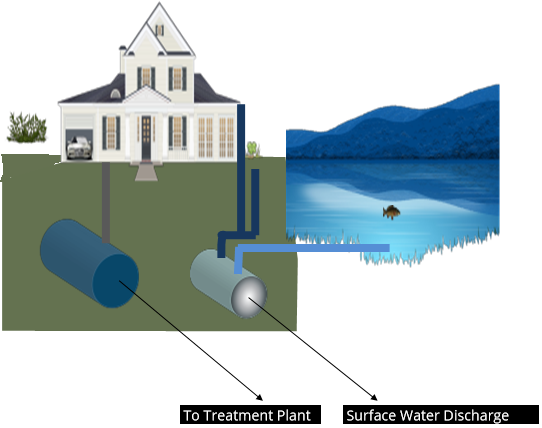
\includegraphics[scale=0.45]{SeperatedSystem1} \hspace{1 cm} 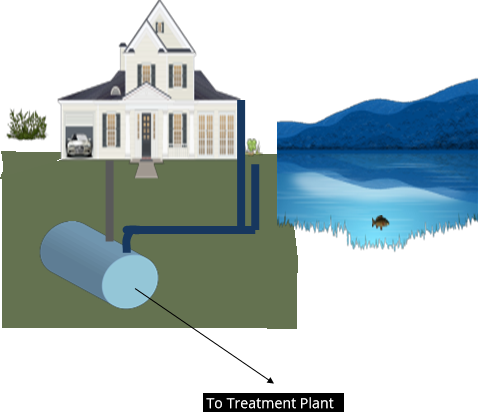
\includegraphics[scale=0.45]{CombinedSystem1}
\end{center}
			\hspace{2.6cm} Separated System \hspace{3.2cm} \parbox{\textwidth}{Combined System}\\

\subsection{Treatment}\index{Treatment}

\begin{itemize}
\item Wastewater treatment can involve physical, chemical or biological processes or combinations of these processes depending on the required outflow standards. 
\item Wastewater treatment typically involves a series of steps with increasing level of treatment:
\begin{itemize}
\item \hl{Preliminary}:  The preliminary process removes large/coarse solids which include rocks, tree branches, grit and other debris present in wastewater.
\item \hl{Primary}:  The primary process is also a physical process where the separable wastewater solids - solids that float and solids that can settle, are removed.  
\item \hl{Secondary}:  Secondary treatment is a biological treatment process where microorganisms consume the organic matter present in the wastewater. 
\item \hl{Tertiary or Advanced Treatment}:  The tertiary/advanced treatment processes improve the quality of treated water beyond the secondary treatment level.  This process may include nutrient removal and disinfection.

\item Solids treatment processes are primarily geared to ensure that the solids generated as part of the wastewater treatment processes, meet the federal regulatory requirements established for wastewater generated solids, at the lowest cost and environmental impact.
\end{itemize}

A generalized layout/process sequencing in a wastewater treatment plant is shown below:
\begin{center}
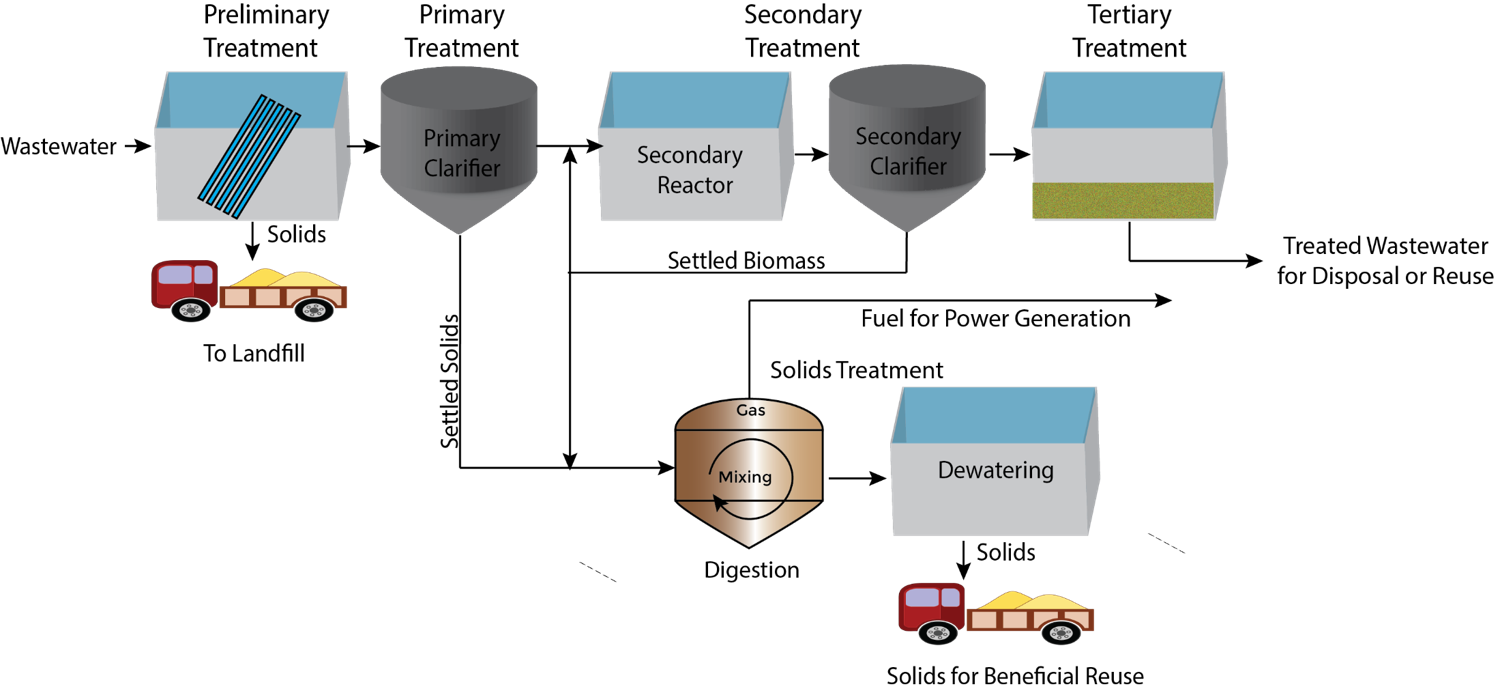
\includegraphics[scale=0.6]{TreatmentFlow}
\end{center}
Individual wastewater treatment processes involve different process options or sequences which are illustrated in the graphic below:
\begin{center}
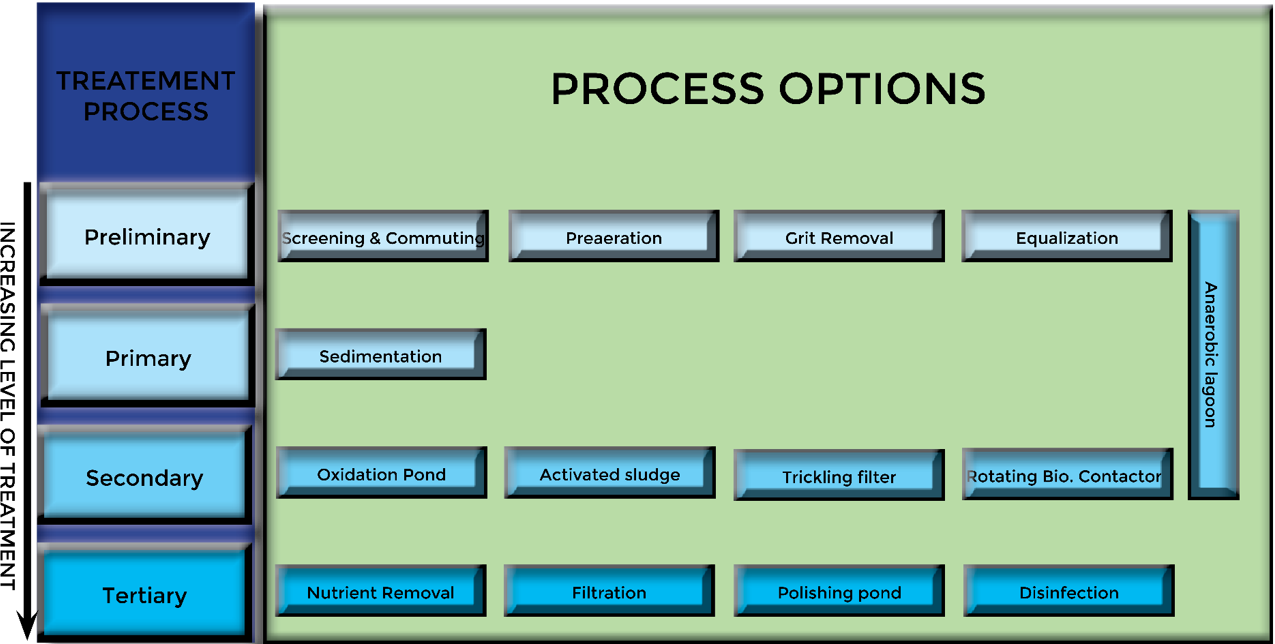
\includegraphics[scale=0.42]{Treatment}
\end{center}
\end{itemize}

\subsection{Disposal or Reuse}\index{Disposal or Reuse}

\begin{itemize}
\item Wastewater treatment processes can be designed to \hl{dispose} the treated water where the water is reintroduced to the environment or for \hl{reuse} where the treated water is \hl{reclaimed} or \hl{recycled} - for various purposes including irrigation, industrial use or for potable use.
\item Water disposal methods include:\\
\begin{itemize}
\item \hl{Surface water discharge}
\item \hl{Subsurface discharge}
\end{itemize}
\item Water reuse methods include:\\
\begin{itemize}
\item Potable water reuse
\begin{itemize}
\item \hl{Indirect potable reuse:}  Here the treated water is blended with groundwater or surface water and then reclaimed and treated further 
for drinking (potable) water use
\item \hl{Direct potable reuse:}  Here the treated wastewater is subjected to advanced treatment and introduced directly into a municipal water supply system
\end{itemize}
\item Water reclamation for irrigation or industrial use\\
\item Land application for beneficial use\\
\end{itemize}
\item Solids generated from the wastewater treatment process may be removed and disposed to a landfill or subject to further treatment which may allow for energy recovery - from the organic solids and for beneficial reuse due to its plant nutrient content.\\
\end{itemize}

\section{New View of Wastewater Treatment}\index{New View of Wastewater Treatment}
Wastewater generation is an inevitable outcome of human existence and its treatment evolved from the basic need for human survival - sanitation.  An increasing awareness of wastewater treatment's environmental and economic impacts, coupled with the very observable effects of global climate changes, there is a move underway to transform Wastewater Treatment Facilities (WWTF) to Renewable Resource Recovery Facilities (RRRF) or Water Resource Recovery Facilities (WRRF) - one which focuses on harnessing it to produces clean water, recover energy and generate nutrients.  



%\chapterimage{MathCover.png} % Chapter heading image
%\chapter{Wastewater Math}
%
%
%% \begin{enumerate}
%% \definecolor{shadecolor}{RGB}{200, 200, 240}
%% \begin{snugshade*}
%%\section{Units and Unit Conversion}\index{Units and Unit Conversion}
%% 	\item \noindent\textsc{Units and Unit Conversion}
%% \end{snugshade*}
%\section{Unit Conversions}\index{Unit Conversions}
%For converting one measurement unit to another.
%
%Step 1:  \texthl{Make sure the original unit is for the same measurement as the converted (desired) unit.}  So if the original unit is for area, say in ft$^2$ the converted unit should be another area unit such as in$^2$ or acre but it cannot be gallons as gallon is a unit of volume.
%
%Step 2: Write down the conversion formula as:
%
%$Quantity \enspace in \enspace converted \enspace unit = Quantity \enspace (\cancel{Original \enspace Unit}) *   Conversion  \enspace Factor \enspace  \dfrac{Conversion \enspace unit}{\cancel{Original \enspace unit}}$
%
%
%\begin{table}[h!]
%
%\begin{center}
%    \begin{tabular}{ | p{4cm} |p{8cm}|}
%    \hline
%    
%    
%Length  & inches, ft, miles\\
%\hline 
%Area  & ft$^2$, acres \\
%\hline 
%Volume & ft$^3$, gallons, acres-ft.\\
%\hline 
%Density & weight per volume, lbs/ft$^3$, lbs/gallon\\
%\hline 
%Flow & ft$^3$/min, MGD, acres-ft/day\\
%\hline 
%
%	
%
%    \end{tabular}
% \caption{Common units in wastewater calculations}	
%    \end{center}
%
%    \end{table}
%
%
%
%\section{Example Problems}
%Problem 1\\
%Convert 1000 $ft^3$ to cu. yards\\
%
%$1000 \cancel{ft^3}*\dfrac{cu.yards}{27\cancel{ft^3}} = 37 cu.yards$
%
%Problem 2\\
%Convert 10 gallons/min to $ft^3$/hr\\
%
%$\dfrac{10 \cancel{gallons}}{\cancel{min}}*  \dfrac{ft^3}{7.48 \cancel{gallons}}  * \dfrac{60 \cancel{min}}{hr}   = \dfrac{80.2ft^3}{hr}$
%
%
%Problem 3\\
%Convert 100,000 $ft^3$ to acre-ft.\\
%$100,000 \cancel{ft^3} * \dfrac{acre-ft}{43,560 \cancel{ft^2-ft}} =  2.3 acre-ft$\\
%\textbf{Note:} From the conversion table: acre = 43,560 $ft^2$\\
%Thus, acre-ft  = 43,560 $ft^2$-ft\\
%
%\section{Pounds Formula}\index{Pounds Formula}
%%\section{Pounds Formula}\index{Pounds Formula}
%
%% \begin{snugshade*}
%% \item \noindent\textsc{Pounds Formula}
%% \end{snugshade*}
%Pounds formula is used for:
%\begin{itemize}
%\item Calculating the quantity in pounds of a particular wastewater constituent entering or leaving a wastewater treatment process
%\item Calculating the pounds of chemicals to be added\\
%\end{itemize}
%So if the concentration of a particular constituent (in mg/liter) and the volume or flow of wastewater is given, one can calculate the amount of that constituent in pounds using the following – Pounds Formula:
%$$lbs \enspace \textbf{or} \enspace \dfrac{lbs}{day}=Concentration\Big(\frac{mg}{l}\Big)*8.34*volume(MG) \enspace \textbf{or} \enspace Flow (MGD)$$\\
%
%The Davidson Pie as shown below provides a pictorial representation of the Pounds Formula.
%
%	\begin{figure}[H]
%\begin{center}
%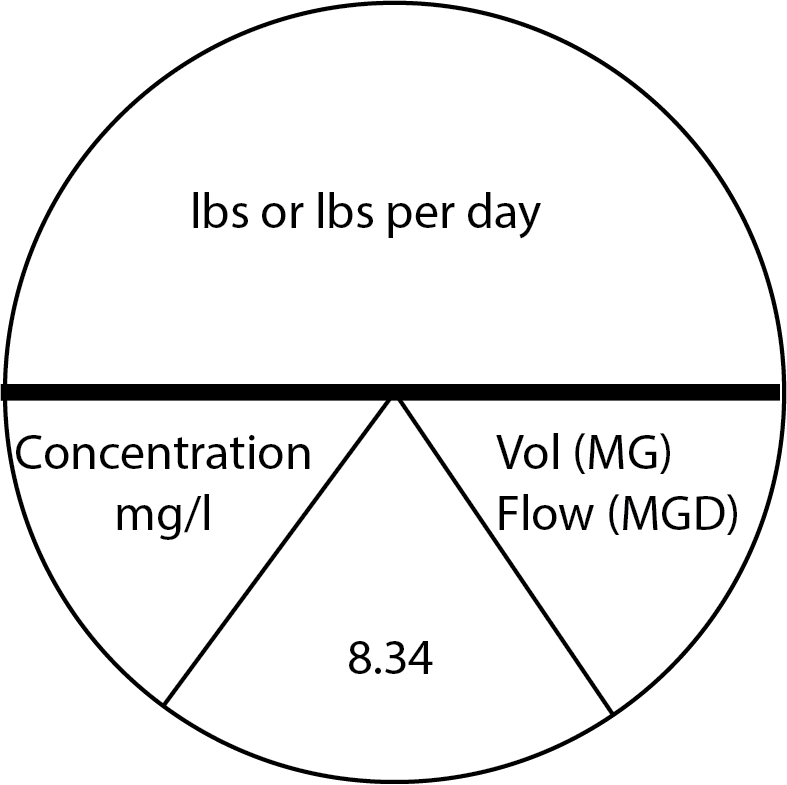
\includegraphics[scale=0.5]{PoundsFormula}
%\end{center}
%\caption{Davidson Pie}
%\end{figure}
%
%In the Pounds Formula, there are three variables – lbs, concentration and volume, and one constant - 8.34.  Knowing any of the two variables in the formula, one can calculate the third (unknown) variable by rearranging the equation.\\
%
%\vspace{0.3cm}
%Davidson Pie provides a pictorial reference for calculating any unknown variable.  If for example, if Concentration is unknown, it can be calculated as follows: \\$$Concentration\Big(\frac{mg}{l}\Big)=\dfrac{lbs \enspace \textbf{or} \enspace \dfrac{lbs}{day}}{8.34*Volume(MG) \enspace \textbf{or} \enspace Flow (MGD)}$$\\
%
%\vspace{0.3cm}
%
%Likewise, if Volume (or Flow) is the unknown variable. it can be calculated as:  \\$$Volume (MG) \enspace or \enspace Flow(MGD)=\dfrac{lbs \enspace \textbf{or} \enspace \dfrac{lbs}{day}}{Concentration\Big(\dfrac{mg}{l}\Big)* \enspace 8.34  }$$
%\newpage
%\section{Concentration}\index{Concentration}
%
%Concentration is typically expressed as mg/l which is the weight of the constituent (mg) in 1 l (liter) of solution (wastewater).  As 1 l of water weighs 1 million mg, a concentration of 1 mg/l implies 1 mg of constituent per 1 million mg of water or one part per million (ppm).   \textbf{Thus, mg/l and ppm are synonymous.}\\  
%Sometimes the constituent concentration is expressed in terms of percentage.\\
%\vspace{6pt}
%For example:  sludge containing 5\% solids or a 12.5\% chlorine concentration solution.\\
%\vspace{6pt}
%As one liter of water weighs 1,000,000 mg, one percent of that weight is 10,000 mg.  So 1\% solids implies 10,000 mg of solids per liter or 10,000 mg/l or 10,000 ppm.\\
%\vspace{6pt}
%$1\% \enspace concentration = 10,000 \enspace ppm \enspace or \enspace\dfrac{mg}{l}$\\
%$0.1\% \enspace concentration = 1,000 \enspace ppm \enspace or \enspace \dfrac{mg}{l}$\\
%$0.01\% \enspace concentration = 100 \enspace ppm \enspace or \enspace \dfrac{mg}{l}$\\
%$10\% \enspace concentration = 100,000 \enspace ppm \enspace or \enspace \dfrac{mg}{l}$\\
%$5\% \enspace concentration = 50,000 \enspace ppm \enspace or \enspace \dfrac{mg}{l}$\\
%$12.5\% \enspace concentration = 125,000 \enspace ppm \enspace or \enspace \dfrac{mg}{l}$\\
%
%\subsection{Example Problems}
%% \hl{Example Problems}\\
%
%Problem 1\\Calculate the lbs/day of solids entering the plant given the influent flow is 5 MGD with an average solids concentration  of 250 mg/l.\\
%
%Solution\\
%
%Applying lbs formula:\\
%$\dfrac{lbs}{day}=5 MGD *250\dfrac{mg}{l}*8.34 = \boxed{10,425\dfrac{lbs}{day}}$
%\\
%\vspace{6pt}
%Problem 2\\Calculate the lbs of solids in the primary sludge if the sludge flow is 7500 gallons and the solids concentration is 4.5\%.\\
%Solution\\
%Applying lbs formula:\\
%$lbs \enspace solids = \dfrac{7500}{1,000,000}MG * 4.5*10,000 *8.34 = \boxed{2,815 \enspace lbs \enspace solids}$\\
%\textbf{Note:}\\  
%1) 7500 gallons was converted to MG by dividing by 1,000,000\\
%$7500 \enspace gallons * \dfrac{1 MG}{1,000,000 \enspace gallon}$\\
%2) 4.5\% was converted to mg/l by multiplying by 10,000 as 1\%=10,000mg/l
%
%
%\section{Area \& Volume}\index{Area \& Volume}
%% \section{Area \& Volume}\index{Area \& Volume}
%
%% \begin{snugshade*}
%% 	\item \noindent\textsc{Area \& Volume}
%% \end{snugshade*}
%
%\begin{center}
%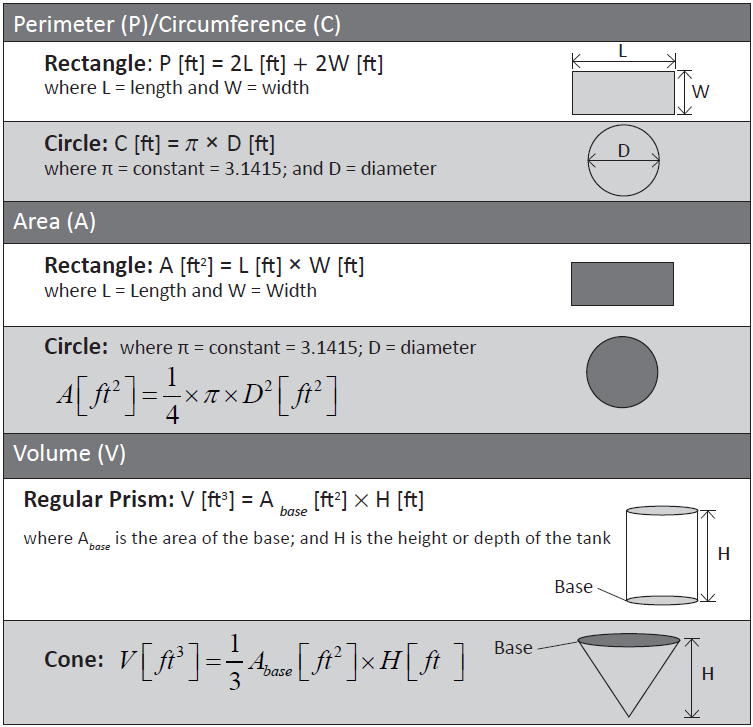
\includegraphics[scale=0.5]{Area&VolumeFormula}
%\end{center}
%\subsection{Example Problems}
%% \hl{Example Problems}\\
%\begin{enumerate}
%
%\item The floor of a rectangular building is 20 feet long by 12 feet wide and the inside walls are 10 feet high. Find the total surface area of the inside walls of this building\\
%Solution:\\
%% \begin{center}
%\begin{tikzpicture}
%	%%% Edit the following coordinate to change the shape of your
%	%%% cuboid
%      
%	%% Vanishing points for perspective handling
%	\coordinate (P1) at (-7cm,1.5cm); % left vanishing point (To pick)
%	\coordinate (P2) at (8cm,1.5cm); % right vanishing point (To pick)
%
%	%% (A1) and (A2) defines the 2 central points of the cuboid
%	\coordinate (A1) at (0em,0cm); % central top point (To pick)
%	\coordinate (A2) at (0em,-2cm); % central bottom point (To pick)
%
%	%% (A3) to (A8) are computed given a unique parameter (or 2) .8
%	% You can vary .8 from 0 to 1 to change perspective on left side
%	\coordinate (A3) at ($(P1)!.8!(A2)$); % To pick for perspective 
%	\coordinate (A4) at ($(P1)!.8!(A1)$);
%
%	% You can vary .8 from 0 to 1 to change perspective on right side
%	\coordinate (A7) at ($(P2)!.7!(A2)$);
%	\coordinate (A8) at ($(P2)!.7!(A1)$);
%
%	%% Automatically compute the last 2 points with intersections
%	\coordinate (A5) at
%	  (intersection cs: first line={(A8) -- (P1)},
%			    second line={(A4) -- (P2)});
%	\coordinate (A6) at
%	  (intersection cs: first line={(A7) -- (P1)}, 
%			    second line={(A3) -- (P2)});
%
%	%%% Depending of what you want to display, you can comment/edit
%	%%% the following lines
%
%	%% Possibly draw back faces
%
%	\fill[gray!40] (A2) -- (A3) -- (A6) -- (A7) -- cycle; % face 6
%	\node at (barycentric cs:A2=1,A3=1,A6=1,A7=1) {\tiny Floor=W*L};
%	
%	\fill[gray!50] (A3) -- (A4) -- (A5) -- (A6) -- cycle; % face 3
%	\node at (barycentric cs:A3=1,A4=1,A5=1,A6=1) {\tiny Wall - W*H};
%	
%	\fill[gray!10, opacity=0.2] (A5) -- (A6) -- (A7) -- (A8) -- cycle; % face 4
%	\node at (barycentric cs:A5=1,A6=1,A7=1,A8=1) {\tiny Wall - L*H};
%	
%	\fill[gray!10,opacity=0.5] (A1) -- (A2) -- (A3) -- (A4) -- cycle; % f2
%	\node at (barycentric cs:A1=1,A2=1,A3=1,A4=1) {\tiny Wall - L*H};
%	
%	\fill[gray!40,opacity=0.2] (A1) -- (A4) -- (A5) -- (A8) -- cycle; % f5
%	\node at (barycentric cs:A1=1,A4=1,A5=1,A8=1) {\tiny Ceiling=W*L};	
%	
%	\draw[thick,dashed] (A5) -- (A6);
%	\draw[thick,dashed] (A3) -- (A6);
%	\draw[thick,dashed] (A7) -- (A6);
%
%	%% Possibly draw front faces
%
%	%\fill[orange] (A1) -- (A8) -- (A7) -- (A2) -- cycle; % face 1
%	\node at (barycentric cs:A1=1,A8=1,A7=1,A2=1) {\tiny Wall - W*H};
%	
%
%
%	%% Possibly draw front lines
%	\draw[thick] (A1) -- (A2);
%
%	\draw[<->] (-1.8,0.38) -- (-1.8,-1.3)node [midway, above=-1.8mm] {\hspace{-1.3cm}\tiny Height=10'};
%	\draw[<->] (-1.6,-1.4) -- (-.3,-2.1)node [midway, above=-2.6mm] {\hspace{-1.3cm}\tiny Length=20'};
%	\draw[<->] (2.6,-1.13) -- (0.2,-2.2)node [midway, below=.6mm] {\hspace{1.2cm}\tiny Width=12'};
%	\draw[thick] (A3) -- (A4);
%	\draw[thick] (A7) -- (A8);
%	\draw[thick] (A1) -- (A4);
%	\draw[thick] (A1) -- (A8);
%	\draw[thick] (A2) -- (A3);
%	\draw[thick] (A2) -- (A7);
%	\draw[thick] (A4) -- (A5);
%	\draw[thick] (A8) -- (A5);
%	
%	% Possibly draw points
%	% (it can help you understand the cuboid structure)
%%	\foreach \i in {1,2,...,8}
%%	{
%%	  \draw[fill=black] (A\i) circle (0.15em)
%%	    node[above right] {\tiny \i};
%%	}
%	% \draw[fill=black] (P1) circle (0.1em) node[below] {\tiny p1};
%	% \draw[fill=black] (P2) circle (0.1em) node[below] {\tiny p2};
%\end{tikzpicture}\\
%% \end{center}
%2 Walls W*H + 2 Walls L*H= $2*12*10ft^2 + 2*20*10ft^2$\\
%$=240+400=\boxed{640ft^2}$\\
%
%2 Walls W*H + 2 Walls L*H + Floor + Ceiling= $2*12*10ft^2 + 2*20*10ft^2 + 2*12*20ft^2$\\
%$=240+400+480=\boxed{1,120ft^2}$\\
%
%\item How many gallons of paint will be required to paint the inside walls of a 40 ft long x 65 ft wide x 20 ft high tank if the paint coverage is 150 sq. ft per gallon.  Note:  We are painting walls only.  Disregard the floor and roof areas.\\
%Solution:\\
%\vspace{0.3cm}
%% \begin{center}
%\begin{tikzpicture}
%	%%% Edit the following coordinate to change the shape of your
%	%%% cuboid
%      
%	%% Vanishing points for perspective handling
%	\coordinate (P1) at (-7cm,1.5cm); % left vanishing point (To pick)
%	\coordinate (P2) at (8cm,1.5cm); % right vanishing point (To pick)
%
%	%% (A1) and (A2) defines the 2 central points of the cuboid
%	\coordinate (A1) at (0em,0cm); % central top point (To pick)
%	\coordinate (A2) at (0em,-2cm); % central bottom point (To pick)
%
%	%% (A3) to (A8) are computed given a unique parameter (or 2) .8
%	% You can vary .8 from 0 to 1 to change perspective on left side
%	\coordinate (A3) at ($(P1)!.8!(A2)$); % To pick for perspective 
%	\coordinate (A4) at ($(P1)!.8!(A1)$);
%
%	% You can vary .8 from 0 to 1 to change perspective on right side
%	\coordinate (A7) at ($(P2)!.7!(A2)$);
%	\coordinate (A8) at ($(P2)!.7!(A1)$);
%
%	%% Automatically compute the last 2 points with intersections
%	\coordinate (A5) at
%	  (intersection cs: first line={(A8) -- (P1)},
%			    second line={(A4) -- (P2)});
%	\coordinate (A6) at
%	  (intersection cs: first line={(A7) -- (P1)}, 
%			    second line={(A3) -- (P2)});
%
%	%%% Depending of what you want to display, you can comment/edit
%	%%% the following lines
%
%	%% Possibly draw back faces
%
%	\fill[gray!40] (A2) -- (A3) -- (A6) -- (A7) -- cycle; % face 6
%	\node at (barycentric cs:A2=1,A3=1,A6=1,A7=1) {};
%	
%	\fill[gray!50] (A3) -- (A4) -- (A5) -- (A6) -- cycle; % face 3
%	\node at (barycentric cs:A3=1,A4=1,A5=1,A6=1) {\tiny Wall - W*H};
%	
%	\fill[gray!10, opacity=0.2] (A5) -- (A6) -- (A7) -- (A8) -- cycle; % face 4
%	\node at (barycentric cs:A5=1,A6=1,A7=1,A8=1) {\tiny Wall - L*H};
%	
%	\fill[gray!10,opacity=0.5] (A1) -- (A2) -- (A3) -- (A4) -- cycle; % f2
%	\node at (barycentric cs:A1=1,A2=1,A3=1,A4=1) {\tiny Wall - L*H};
%	
%	\fill[gray!40,opacity=0.2] (A1) -- (A4) -- (A5) -- (A8) -- cycle; % f5
%	\node at (barycentric cs:A1=1,A4=1,A5=1,A8=1) {};	
%	
%	\draw[thick,dashed] (A5) -- (A6);
%	\draw[thick,dashed] (A3) -- (A6);
%	\draw[thick,dashed] (A7) -- (A6);
%
%	%% Possibly draw front faces
%
%	%\fill[orange] (A1) -- (A8) -- (A7) -- (A2) -- cycle; % face 1
%	\node at (barycentric cs:A1=1,A8=1,A7=1,A2=1) {\tiny Wall - W*H};
%	
%
%
%	%% Possibly draw front lines
%	\draw[thick] (A1) -- (A2);
%
%	\draw[<->] (-1.8,0.38) -- (-1.8,-1.3)node [midway, above=-1.8mm] {\hspace{-1.3cm}\tiny Height=20'};
%	\draw[<->] (-1.6,-1.4) -- (-.3,-2.1)node [midway, above=-2.6mm] {\hspace{-1.3cm}\tiny Length=40'};
%	\draw[<->] (2.6,-1.13) -- (0.2,-2.2)node [midway, below=.6mm] {\hspace{1.2cm}\tiny Width=65'};
%	\draw[thick] (A3) -- (A4);
%	\draw[thick] (A7) -- (A8);
%	\draw[thick] (A1) -- (A4);
%	\draw[thick] (A1) -- (A8);
%	\draw[thick] (A2) -- (A3);
%	\draw[thick] (A2) -- (A7);
%	\draw[thick] (A4) -- (A5);
%	\draw[thick] (A8) -- (A5);
%	
%	% Possibly draw points
%	% (it can help you understand the cuboid structure)
%%	\foreach \i in {1,2,...,8}
%%	{
%%	  \draw[fill=black] (A\i) circle (0.15em)
%%	    node[above right] {\tiny \i};
%%	}
%	% \draw[fill=black] (P1) circle (0.1em) node[below] {\tiny p1};
%	% \draw[fill=black] (P2) circle (0.1em) node[below] {\tiny p2};
%\end{tikzpicture}\\
%% \end{center}
%\vspace{0.3cm}
%2 Walls W*H + 2 Walls L*H = $2*65*20ft^2 + 2*40*20ft^2= 2,600+1,600=4,200ft^2$\\
%$\implies @150\dfrac{ft^2}{gal} \enspace paint \enspace coverage \enspace \rightarrow \enspace \dfrac{4,200\cancel{ft^2}}{150\dfrac{\cancel{ft^2}}{gal}}=\boxed{28 \enspace gallons}$
%\vspace{0.3cm}
%\item What is the circumference of a 100 ft diameter circular clarifier?\\
%\vspace{0.3cm}
%Solution:\\
%\vspace{0.3cm}
%$Circumference=\pi*D=3.14*100ft=\boxed{314ft}$
%\vspace{0.3cm}
%\item If the surface area of a clarifier is 5,025$ft^2$, what is its diameter?\\
%\vspace{0.3cm}
%Solution:\\
%\vspace{0.3cm}
%$Surface \enspace area=\dfrac{\pi}{4}*D^2 \enspace \implies 5025(ft^2)=0.785*D^2 (ft^2)$\\
%$\implies D^2=\dfrac{5025}{0.785} \implies D=\sqrt{6401.3}=\boxed{80ft}$
%\vspace{0.3cm}
%
%\item How many gallons of wastewater would 600 feet of 6-inch diameter pipe hold, approximately?\\
%\vspace{0.3cm}
%Solution:\\
%
%\vspace{0.3cm}
%% \begin{center}
%\begin{tikzpicture}
%\draw (0,0) ellipse (0.1cm and 0.3cm);
%\draw (10,0) ellipse (0.1cm and 0.3cm);
%\draw [-] (0,-0.29) -- (10,-0.29);
%\draw [-] (0,0.29) -- (10,0.29);
%\draw [<->] (10,-0.28) -- (10,0.28) node [midway, below=-3mm] {\hspace{2.6cm}Diameter=6"};
%\draw [<->] (0,-.68) -- (10,-.68)node [midway, below] {\hspace{0.9cm}Length=600'};
%\end{tikzpicture}
%% \end{center}
%\vspace{0.3cm}
%$Volume=\dfrac{\pi}{4}D^2*L=0.785*\Big(\dfrac{6}{12}\Big)^2*600\cancel{ft^3}*7.48\dfrac{gallons}{\cancel{ft^3}}=\boxed{881 \enspace gallons}$
%\vspace{0.5cm}
%\item A 110 ft diameter digester with a 12 ft deep cone is operated at a side water depth of 20 ft.  Caluclate the volume of sludge in the digester in $ft^3$ and gallons.\\
%\vspace{0.3cm}
%Solution:\\
%\vspace{0.3cm}
%% \begin{center}
%\begin{tikzpicture}
%\draw (0,0) ellipse (2cm and 0.3cm);
%\draw (0,-2.3) ellipse (2cm and 0.3cm);
%\draw (0,-.8) ellipse (2cm and 0.3cm);
%\draw [-] (2,-2.3) -- (2,0);
%\draw [<->] (-2,0) -- (2,0) node [midway, below=-0.9cm] {\hspace{0.9cm}Diameter (D)=110'}; 
%\draw [<->] (-2.6,-2.3) -- (-2.6,0) node [midway, below=-.3cm] {\hspace{-2.6cm}Cylinder Height};
%\draw [<->] (2.5,-2.3) -- (2.5,-0.8) node [midway, below=-0.2cm] {\hspace{5.2cm}Side Water Depth (SWD) =20'};
%\draw [-] (0,-4) -- (2,-2.3);
%\draw [-] (0,-4) -- (-2,-2.3);
%\draw [-] (0,-4) -- (2,-2.3);
%\draw [-] (-2,0) -- (-2,-2.3);
%\draw [<->] (2.5,-2.3) -- (2.5,-4)node [midway, below=-0.4cm] {\hspace{3.8cm}Cone Depth (CD)=12'};
%\end{tikzpicture}\\
%% \end{center}
%$Digester \enspace volume=Volume_{cylinder}+Volume_{cone}$\\
%$\implies Digester \enspace volume=\dfrac{\pi}{4}D^2*SWD+\dfrac{1}{3}*\Bigg(\pi*D^2*CD\Bigg)$\\
%\vspace{0.3cm}
%$=0.785*110^2*20+1.05*110^2*12=\boxed{227,988ft^3}$\\
%\vspace{0.3cm}
%$227,988\cancel{ft^3}*7.48\dfrac{gallons}{\cancel{ft^3}}=\boxed{1,705,352 \enspace gallons}$
%\end{enumerate}
%
%\section{Process Removal Efficiency}\index{Process Removal Efficiency}
%
%% \section{Process Removal Efficiency}\index{Process Removal Efficiency}
%% \begin{snugshade*}
%% 	\item \noindent\textsc{Process Removal Efficiency}
%% \end{snugshade*}
%\begin{itemize}
%\item Process removal rate or removal efficiency is the percentage of the inlet concentration removed.  
%\item It is used for quantifying the pollutant removal during wastewater treatment and is established based upon the amount of a particular wastewater constituent entering and leaving a treatment process.
%
%\item $Process \enspace Removal \enspace Rate \enspace (\%) = \dfrac{Pollutant \enspace  In-Pollutant\enspace  Out}{Pollutant \enspace In}*100$\\
%
%\item If 10 units of a pollutant are entering a process and 8 units of pollutant are leaving (process removes 2 units), then the process removal rate for that pollutant is (10-8)/10*100=20\%.  In this example the process is 20\% efficient in removing that particular pollutant.
%
%\item The amount of pollutant can be measured in terms of concentration (mg/l) or in terms of mass loading (lbs).  The pounds formula is used for calculating the mass loadings.  
%\end{itemize}
%The above example is for calculating the removal efficiency using the inlet and outlet concentrations or mass loading.\\
%The methods below can be used for calculating either the inlet or outlet pollutant concentrations, if the removal efficiency and the corresponding inlet or outlet concentrations are given. 
%
%
%\hl{Case 1:  Calculating outlet conc. (X) given the inlet conc. and removal efficiency (RE\%):}
%
%\tikzstyle{block} = [rectangle, draw, fill=red!40, 
%    text width=6em, text centered, rounded corners, minimum height=3em]
%\tikzstyle{arrow} = [draw, -latex']
%\begin{figure}[!h]
%\centering
%\begin{tikzpicture}[node distance =1.5cm, auto]
%    \draw ++(0,0) node [block] (Process) {Process};
%   \node[node distance=1.9in] (dummy_in) [left of=Process] {In};
%   \node[node distance=1.9in] (dummy_out) [right of=Process] {Out};
%	\node (Removal) [below of=Process, yshift=-0in] {${Removal \enspace Efficiency=RE\% \enspace (Given)}$};
%    \path [arrow] (dummy_in)-- (Process)  node [above] {\hspace{-5.8cm}$A \enspace mg/l \enspace (Given) $} node [below] {\hspace{-5.8cm}$100 \enspace mg/l$};
%    \path [arrow] (Process) -- (dummy_out)  node [above] {\hspace{-4cm}$X \enspace mg/l \enspace (Unknown)$} node [below] {\hspace{-3.9cm}($100-RE\%)\enspace mg/l$};
%   \draw[arrow] (Process) -- (Removal);
%\end{tikzpicture}
%\end{figure}
%Using the fact that if the inlet concentration was 100 mg/l, the outlet concentration would be 100 minus the removal efficiency.\\
%Setup the equation as:  $\dfrac{Out}{In}: \enspace \dfrac{X \enspace mg/l}{A \enspace mg/l}=\dfrac{100-RE\%}{100}$\\
%Calculate X using cross multiplication - if $\dfrac{A}{B}=\dfrac{C}{D} \implies A=B*\dfrac{C}{D}$:\\
%$X \enspace mg/l=A \enspace mg/l*\dfrac{100-RE\%}{100}$\\
%
%
%\hl{Case 2:  Calculating inlet conc. (X) given the outlet conc. and removal efficiency (RE\%):}
%
%\begin{figure}[!h]
%\centering
%\begin{tikzpicture}[node distance =1.5cm, auto]
%    \draw ++(0,0) node [block] (Process) {Process};
%   \node[node distance=1.9in] (dummy_in) [left of=Process] {In};
%   \node[node distance=1.9in] (dummy_out) [right of=Process] {Out};
%	\node (Removal) [below of=Process, yshift=-0in] {$Removal \enspace Efficiency=RE\% \enspace (Given)$};
%    \path [arrow] (dummy_in)-- (Process)  node [above] {\hspace{-5.8cm}$X \enspace mg/l \enspace (Unknown)$} node [below] {\hspace{-5.8cm}$100 \enspace mg/l$};
%    \path [arrow] (Process) -- (dummy_out)  node [above] {\hspace{-4cm}$A \enspace mg/l \enspace (Given)$} node [below] {\hspace{-3.9cm}($100-RE\%)\enspace mg/l$};
%   \draw[arrow] (Process) -- (Removal);
%\end{tikzpicture}
%\end{figure}
%Using the fact that if the inlet concentration was 100 mg/l, the outlet concentration would be 100 minus the removal efficiency.\\
%Setup the equation as:  $\dfrac{In}{Out}: \enspace \dfrac{X \enspace mg/l}{A \enspace mg/l}=\dfrac{100}{100-RE\%}$\\
%\vspace{0.3cm}
%Calculate X using cross multiplication - if $\dfrac{A}{B}=\dfrac{C}{D} \implies A=B*\dfrac{C}{D}$:\\
%$X \enspace mg/l=A \enspace mg/l*\dfrac{100}{100-RE\%}$\\
%
%\vspace{0.4cm}
%\subsection{Example Problems}
%% \hl{Example Problems:}\\
%
%\begin{enumerate}
%
%\item What is the \% removal efficiency if the influent concentration is 10 mg/L and the effluent concentration is 2.5 mg/L?\\
%$Removal \enspace Rate (\%) = \dfrac{In-Out}{In}*100 \implies \dfrac{10-2.5}{10}*100=\boxed{75\%}$
%
%
%
%\item Calculate the outlet concentration if the inlet concentration is 80 mg/l and the process removal efficiency is 60\%\\
%Solution:\\
%
%\tikzstyle{block} = [rectangle, draw, fill=red!40, 
%    text width=6em, text centered, rounded corners, minimum height=3em]
%\tikzstyle{arrow} = [draw, -latex']
%\begin{figure}[!h]
%\centering
%\begin{tikzpicture}[node distance =1.5cm, auto]
%    \draw ++(0,0) node [block] (Process) {Process};
%   \node[node distance=1.5in] (dummy_in) [left of=Process] {In};
%   \node[node distance=1.5in] (dummy_out) [right of=Process] {Out};
%	\node (Removal) [below of=Process, yshift=-0in] {$Removal \enspace Efficiency=60\%$};
%    \path [arrow] (dummy_in)-- (Process)  node [above] {\hspace{-4.39cm}$80mg/l$} node [below] {\hspace{-4.39cm}$100mg/l$};
%    \path [arrow] (Process) -- (dummy_out)  node [above] {\hspace{-3.cm}$Xmg/l$} node [below] {\hspace{-3cm}40mg/l};
%   \draw[arrow] (Process) -- (Removal);
%\end{tikzpicture}
%%\caption[MFCC]{Diagrama en bloques del cálculo de las MFCC para un frame.}
%%\label{MFCC}
%\end{figure}
%
%$\dfrac{Out}{In} \enspace:\enspace\dfrac{Actual \enspace Outlet (X)}{80}=\dfrac{100-60}{100}$\\
%$\implies \dfrac{Actual \enspace Outlet (X)}{80} =0.4$\\
%$\implies Actual \enspace  Outlet (X) = 0.4 * 80 = \boxed{32 mg/l}$\\
%
%
%\item Calculate the inlet concentration if the outlet concentration is 80 mg/l and the process removal efficiency is 60\%\\
%
%\tikzstyle{block} = [rectangle, draw, fill=red!40, 
%    text width=6em, text centered, rounded corners, minimum height=3em]
%\tikzstyle{arrow} = [draw, -latex']
%\begin{figure}[!h]
%\centering
%\begin{tikzpicture}[node distance =1.5cm, auto]
%    \draw ++(0,0) node [block] (Process) {Process};
%   \node[node distance=1.5in] (dummy_in) [left of=Process] {In};
%   \node[node distance=1.5in] (dummy_out) [right of=Process] {Out};
%	\node (Removal) [below of=Process, yshift=-0in] {$Removal \enspace Efficiency=60\%$};
%    \path [arrow] (dummy_in)-- (Process)  node [above] {\hspace{-4.39cm}$Xmg/l$} node [below] {\hspace{-4.39cm}$100mg/l$};
%    \path [arrow] (Process) -- (dummy_out)  node [above] {\hspace{-3.cm}80mg/l} node [below] {\hspace{-3cm}40mg/l};
%   \draw[arrow] (Process) -- (Removal);
%\end{tikzpicture}
%\end{figure}
%
%$\dfrac{In}{Out} \enspace : \enspace \dfrac{Actual \enspace inlet \enspace  (X)}{80}=\dfrac{100}{100-60}\implies \dfrac{Actual \enspace inlet \enspace  (X)}{80}=2.5$\\    
%Rearranging the equation:   $Actual \enspace inlet (X)=2.5*80 = \boxed{200 mg/l}$\\
%
%\item If a plant removes 35\% of the influent BOD in the primary treatment and 85\% of the remaining BOD in the secondary system, what is the BOD of the raw wastewater if the BOD of the final effluent is 20mg/l\\
%Solution:\\
%
%\begin{figure}[!h]
%\centering
%\begin{tikzpicture}[node distance =1.5cm, auto]
%    \draw ++(0,0) node [block] (Primary) {Primary};
%    
%   \node[node distance=1.9in] (dummy_in) [left of=Primary] {Influent BOD};
%   \node[node distance=1.9in] (dummy_out) [right of=Primary] {Primary BOD Out};
%	\node (Removal) [below of=Primary, yshift=-0in] {$Removal \enspace Efficiency=35\% $};
%    \path [arrow] (dummy_in)-- (Primary)  node [above] {\hspace{-4.8cm}$X \enspace mg/l \enspace$} node [below] {};
%    \path [arrow] (Primary) -- (dummy_out)  node [above] {\hspace{-4.9cm}$0.65X \enspace mg/l$} node [below] {};
%   \draw[arrow] (Process) -- (Removal);
%\end{tikzpicture}
%\end{figure}
%
%
%\begin{figure}[!h]
%\centering
%\begin{tikzpicture}[node distance =1.5cm, auto]
%    \draw ++(0,0) node [block] (Secondary) {Secondary};
%    
%   \node[node distance=1.9in] (dummy_in) [left of=Secondary] {Primary BOD Out};
%   \node[node distance=1.9in] (dummy_out) [right of=Secondary] {Secondary BOD Out};
%	\node (Removal) [below of=Secondary, yshift=-0in] {$Removal \enspace Efficiency=85\% $};
%    \path [arrow] (dummy_in)-- (Secondary)  node [above] {\hspace{-4.8cm}$0.65X \enspace mg/l \enspace$} node [below] {\hspace{-5cm}$100 \enspace mg/l$};
%    \path [arrow] (Secondary) -- (dummy_out)  node [above] {\hspace{-4.9cm}$20 \enspace mg/l$} node [below] {\hspace{-4.9cm}$15 \enspace mg/l$};
%   \draw[arrow] (Process) -- (Removal);
%\end{tikzpicture}
%\end{figure}
%\vspace{0.3cm}
%For the Secondary process:\\
%$\dfrac{In}{Out}: \enspace \dfrac{0.65X}{20}=\dfrac{100}{15} \implies X \enspace mg/l=\dfrac{100*20}{15*0.65}=\boxed{205 \enspace mg/l}$\\
%
%\vspace{0.3cm}
%Alternate Solution \#1
%
%$\xrightarrow[
%				\text{X}\dfrac{mg}{l}
%			]
%			{
%			\text{Influent BOD}
%			}
% \boxed{Primary}
% \xrightarrow[
% 				\text{X-0.35X=X*(1-0.35)=0.65X}\dfrac{mg}{l}
% 			]
% 			{
% 			\text{Primary Effluent BOD}
% 			}
% \boxed{Secondary}
% \xrightarrow[
%				\text{0.65X-0.5525X=(0.65-0.5525)X=0.0975X }
%			 ]
%			{
%			\text{Secondary Effluent BOD}
%			}
%$\\
%\hspace{2.8cm}$\downarrow$ {\tiny(0.35X)BOD Removed}\hspace{3.2cm}$\downarrow$ {\tiny(0.65*0.85)X = 0.5525X BOD Removed}\\
%$\implies 0.0975X=20 \implies X=\dfrac{20}{0.0975}=\boxed{205\dfrac{mg}{l}}$\\
%
%\vspace{0.3cm}
%
%Alternate Solution \#2:\\
%$\xrightarrow[\text{X}\dfrac{mg}{l}]{\text{Influent BOD}}\boxed{Primary}\xrightarrow[\text{0.65X}]{\text{Primary Effluent BOD}}\boxed{Secondary}\xrightarrow[\text{(0.65*0.15)X}]{\text{Secondary Effluent BOD}}$\\
%\hspace{2.8cm}$\downarrow$ {\tiny(0.35X)BOD Removed}\hspace{2.2cm}$\downarrow$ {\tiny(0.65X*0.85)BOD Removed}\\
%
%Primary Effluent BOD = Influent BOD * (1-Primary BOD Removal), and\\
%Secondary Effluent BOD=[Primary Effluent BOD]*(1-Secondary BOD Removal)\\
%Secondary Eff. BOD=[Influent BOD * (1-Primary BOD Removal)]*(1-Secondary BOD Removal)\\
%
%Therefore, 20 = [X*(1-0.35)] * (1-0.85)= X*0.65*0.15\\
%$\implies 20 \enspace \dfrac{mg}{l}= 0.0975X \implies X=\dfrac{20}{0.0975}=\boxed{205 \enspace \dfrac{mg}{l}}$
%
%\end{enumerate}
%\section{Pumping}\index{Pumping}
%% \section{Pumping}\index{Pumping}
%% \pagebreak
%% \begin{snugshade*}
%% 	\item \noindent\textsc{Pumping}
%% \end{snugshade*}
%For Grades I \& II, pumping rate problems include the following:
%% \begin{enumerate}
%% \definecolor{shadecolor}{RGB}{225, 235, 235}
%% \begin{snugshade*}
%% \item \noindent\textsc{Calculating volume pumped in a given time interval given the pump flow rate\\}
%% \end{snugshade*}
%\subsection{Calculating volume pumped given the pump flow rate}\index{Calculating volume pumped given the pump flow rate}
%
%\textbf{Method:\\}
%\hspace{1cm}Step 1. Multiply the pump flow rate by the time interval\\
%\textbf{Make sure:}
%\begin{itemize}
%\item The time units - in the given time interval and in the pump flow rate match
%\end{itemize}
%\subsection{Calculating time to pump a certain volume}\index{Calculating time to pump a certain volume}
%% \begin{snugshade*}
%% \item \noindent\textsc{Calculating time to pump a certain volume given the pump flow rate\\}
%% \end{snugshade*}
%\textbf{Method:}
%\hspace{1cm}Step 1. Calculate the total volume pumped\\
%\hspace{1cm}Step 2.	Divide the total volume by the pump flow rate\\
%\textbf{Make sure:}
%\begin{itemize}
%\item The volume units - in the volume that needs to be pumped and in the pump flow rate match
%\item The time unit in the pump flow rate needs to be converted to the time unit that you need the answer in
%\end{itemize}
%% \end{enumerate}
%
%\section{Example Problems}
%% \hl{Example Problems:}\\
%
%\begin{enumerate}
%
%\item A sludge pump is set to pump 5 minutes each hour. It pumps at the rate of 35 gpm. How many gallons of sludge are pumped each day?\\
%Solution:\\
%$\dfrac{35 \enspace gal \enspace sludge}{\cancel{min}}*\dfrac{5 \enspace \cancel{min}}{\cancel{hr}} *\dfrac{24 \enspace \cancel{hr}}{day}=\boxed{\dfrac{4,200 \enspace gallons}{day}}$\\
%\vspace{0.5cm}
%
%\item A sludge pump operates 5 minutes each 15 minute interval.  If the pump capacity is 60 gpm, how many gallons of sludge are pumped daily?
%
%$\dfrac{60 \enspace gal \enspace sludge}{\xcancel{min}}*\dfrac{5 \enspace \xcancel{min}}{15 \enspace \cancel{min}}*1440\dfrac{\cancel{min}}{day}=\boxed{\dfrac {28,800 \enspace gal \enspace sludge }{day}}$\\
%
%\item Given the tank is 10ft wide, 12 ft long and 18 ft deep tank including 2 ft of freeboard when filled to capacity. How much time (minutes) will be required to pump down this tank to a depth of 2 ft when the tank is at maximum capacity using a 600 GPM pump\\
%Solution:\\
%\vspace{0.5cm}
%
%
%\begin{tikzpicture}
%
%\pgfmathsetmacro{\cubexx}{4}
%\pgfmathsetmacro{\cubeyy}{1.5}
%\pgfmathsetmacro{\cubezz}{2}
%\pgfmathsetmacro{\cubex}{4}
%\pgfmathsetmacro{\cubey}{0.5}
%\pgfmathsetmacro{\cubez}{2}
%\pgfmathsetmacro{\cubexxx}{4}
%\pgfmathsetmacro{\cubeyyy}{4}
%\filldraw [fill=cyan!10!white, draw=black] (0,-\cubey,0) -- ++(-\cubexx,0,0) -- ++(0,-\cubeyy,0) -- ++(\cubexx,0,0) -- cycle ;
%\filldraw [fill=cyan!0!white, draw=black] (0,-\cubey,0) -- ++(0,0,-\cubezz) -- ++(0,-\cubeyy,0) -- ++(0,0,\cubezz) -- cycle;
%\filldraw [fill=cyan!10!white, draw=black] (0,-\cubey,0) -- ++(0,0,-\cubezz) -- ++(0,-\cubeyy,0) -- ++(0,0,\cubezz) -- cycle;
%%\filldraw [fill=cyan!10!white, draw=black] (0,-\cubey,0) -- ++(-\cubexx,0,0) -- ++(0,0,-\cubezz) -- ++(\cubexx,0,0) -- cycle;
%%%%\draw (0,-0.5,0) -- ++(-\cubex,0,0) -- ++(0,-\cubey,-\cubez) -- ++(\cubex,0,0) -- cycle;
%\draw (-\cubex,0,0) -- ++(0,0,-\cubez) -- ++(0,-\cubey,0) -- ++(0,0,\cubez) -- cycle;
%\draw (0,-\cubey,0) -- ++(-\cubex,0,0) -- ++(0,0,-\cubez) -- ++(\cubex,0,0) -- cycle;
%\filldraw [fill=white, draw=black] (0,0,0) -- ++(-\cubex,0,0) -- ++(0,-\cubey,0) -- ++(\cubex,0,0) -- cycle ;
%\filldraw [fill=white, draw=black] (0,0,0) -- ++(0,0,-\cubez) -- ++(0,-\cubey,0) -- ++(0,0,\cubez) -- cycle;
%\filldraw [fill=white, draw=black] (0,0,0) -- ++(0,0,-\cubez) -- ++(0,-\cubey,0) -- ++(0,0,\cubez) -- cycle;
%\filldraw [fill=white, draw=black] (0,0,0) -- ++(-\cubex,0,0) -- ++(0,0,-\cubez) -- ++(\cubex,0,0) -- cycle;
%
%%\filldraw [fill=RoyalBlue!10!white, draw=black] (0,-1.5,0) -- ++(-\cubex,0,0) -- ++(0,-\cubey,0) -- ++(\cubex,0,0) -- cycle ;
%
%%\filldraw [fill=RoyalBlue!10!white, draw=black] (0,-1.5,0) -- ++(0,0,-\cubez) -- ++(0,-\cubey,0) -- ++(0,0,\cubez) -- cycle;
%
%
%
%%%\draw (0,-0.5,0) -- ++(-\cubex,0,0) -- ++(0,0,-\cubez) -- ++(\cubex,0,0) -- cycle;
%%%\filldraw [fill=white, draw=black] (-\cubex,0,0) -- ++(0,0,-\cubez) -- ++(0,-\cubey,0) -- ++(0,0,\cubez) -- cycle;
%%%\filldraw [fill=white, draw=black] (0,-\cubey,0) -- ++(-\cubex,0,0) -- ++(0,0,-\cubez) -- ++(\cubex,0,0) -- cycle ;
%
%\draw [<->] (-4,-2.3) -- (0,-2.3) node [midway, below] {12' Long};
%\draw [<->] (1,-1.3) -- (1,.2) node [midway, midway] {\hspace{4.5cm}16' Water Depth (Initial)};
%\draw [<->] (0.4,-1.62) -- (0.4,-1.1) node [midway, midway] {\hspace{-4.8cm} 2' Water Depth (Final)};
%\draw [<->] (1,.8) -- (1,.2) node [midway, midway] {\hspace{2.4cm}2' Freeboard};
%\draw [<->] (1,-1.3) -- (0,-2.3) node [midway, midway] {\hspace{2.3cm}10' Wide};
%\end{tikzpicture}\\
%Volume to be pumped=$12 \enspace ft*10 \enspace ft *(16-2)\enspace ft=1,680ft^3$\\
%\vspace{0.3cm}
%$\implies \dfrac{1,680\cancel{ft^3}*7.48\dfrac{\cancel{gal}}{\cancel{ft^3}}}{600\dfrac{\cancel{gal}}{min}}=\boxed{21min}$
%\end{enumerate}
%
%\chapterimage{QuizIcon.jpg}
%\chapter{Week 1 Module Assessment Quiz}
%
%
%
%1. Eutrophication is the degradation of plant and organic matter in a body of water\\
%
%a. True \\
%b. False \\
%\vspace{0.3cm}
%
%2. Direct potable reuse is when advanced treated wastewater is directly introduced into the water supply system\\
%
%a. True \\
%b. False \\
%\vspace{0.3cm}
%
%3. Acre-ft is a measure of volume.\\
%
%a. True \\
%b. False \\
%
%\vspace{0.3cm}
%4. The units ppm and \% are considered roughly equivalent for wastewater treatment calculations.\\
%\vspace{0.3cm}
%a. True \\
%b. False \\
%\vspace{0.3cm}
%
%5. Sludge with a sludge density of 7\% would have a solids concentration of:\\
%
%a. 7 mg/l \\
%b. 700 mg/l \\
%c. 7000 mg/l \\
%d. 70,000 mg/l \\
%
%\vspace{0.3cm}
%6. Convert 1.7 MGD to $ft^3/s$
%\vspace{0.3cm}
%
%
%7. If a primary clarifier consistently operates at 30 \% efficiency and produces an effluent which averages 140 mg/l BOD, what is the influent BOD?\\
%\vspace{0.3cm}
%
%
%8. How long (in minutes) will it take to pump down 25 feet of water in a 110 ft diameter cylindrical tank when using a 1420 gpm pump\\
%
%\vspace{0.3cm}
%
%9. NPDES stands for\\
%
%a. National Pollutant Discharge Elimination System \\
%b. National Permit for Discharge of Effluents \\
%c. Natural Process for Discharge of Effluent Systems \\
%
%\vspace{0.3cm}
%\vspace{26cm}
%
%\textbf{Answers:}\\
%\vspace{0.3cm}
%1.	b.  \\
%
%\vspace{0.3cm}
%2.	a.  \\
%
%\vspace{0.3cm}
%3.	a.  \\
%
%\vspace{0.3cm}
%4.	b.  \\
%\vspace{0.3cm}
%
%5.	d.  \\
%
%\vspace{0.3cm}
%6. Solution:\\
%\vspace{0.3cm}
%$\dfrac{1.7 \cancel{MG}}{\cancel{day}}*  \dfrac{1,000,000 \enspace \cancel{gal}}{\cancel{MG}}*\dfrac{ft^3}{7.48 \cancel{gallons}}  * \dfrac{\cancel{day}}{1,440 *60 sec}   = \boxed{\dfrac{2.63 \enspace ft^3}{s}}$\\
%\vspace{0.3cm}
%7.	Solution:\\
%\vspace{0.3cm}
%Calculate the inlet concentration if the outlet concentration is 80 mg/l and the process removal efficiency is 60\%\\
%
%\tikzstyle{block} = [rectangle, draw, fill=red!40, 
%    text width=6em, text centered, rounded corners, minimum height=3em]
%\tikzstyle{arrow} = [draw, -latex']
%\begin{figure}[!h]
%\centering
%\begin{tikzpicture}[node distance =1.5cm, auto]
%    \draw ++(0,0) node [block] (Process) {Process};
%   \node[node distance=1.5in] (dummy_in) [left of=Process] {In};
%   \node[node distance=1.5in] (dummy_out) [right of=Process] {Out};
%	\node (Removal) [below of=Process, yshift=-0in] {$Removal \enspace Efficiency=30\%$};
%    \path [arrow] (dummy_in)-- (Process)  node [above] {\hspace{-4.39cm}$Xmg/l$} node [below] {\hspace{-4.39cm}$100mg/l$};
%    \path [arrow] (Process) -- (dummy_out)  node [above] {\hspace{-3.cm}140mg/l} node [below] {\hspace{-3cm}70mg/l};
%   \draw[arrow] (Process) -- (Removal);
%\end{tikzpicture}
%\end{figure}
%
%$\dfrac{In}{Out} \enspace : \enspace \dfrac{Actual \enspace inlet \enspace  (X)}{140}=\dfrac{100}{100-30}\implies \dfrac{Actual \enspace inlet \enspace  (X)}{140}=1.43$\\    
%Rearranging the equation:   $Actual \enspace inlet (X)=1.43*140 = \boxed{200 mg/l}$\\
%
%\vspace{0.3cm}
%8.	Solution:\\
%\vspace{0.3cm}
%
%\begin{tikzpicture}
%\draw (0,0) ellipse (2cm and 0.3cm);
%\draw (0,-2.3) ellipse (2cm and 0.3cm);
%\draw [-] (2,-2.3) -- (2,0);
%\draw [<->] (-2,0) -- (2,0) node [midway, above=3mm] {\hspace{0.1cm}Diameter=110'}; 
%\draw [<->] (2.5,-2.3) -- (2.5,0) node [midway, below] {\hspace{1.9cm}Height=25'};
%%\draw [-] (0,-4) -- (2,-2.3);
%%\draw [-] (0,-4) -- (-2,-2.3);
%%\draw [-] (0,-4) -- (2,-2.3);
%\draw [-] (-2,0) -- (-2,-2.3);
%\end{tikzpicture}
%
%\vspace{0.3cm}
%
%$Time=\dfrac{Total \enspace volume \enspace to \enspace be \enspace pumped}{Pump \enspace flow \enspace rate}$
%
%\vspace{0.3cm}
%$\implies \dfrac{(0.785*110^2*25)\cancel{ft^3}*\dfrac{7.48\cancel{gal}}{\cancel{ft^3}}}{\dfrac{1420\cancel{gal}}{min}}= \boxed{1,251 \enspace min}$\\
%
%\vspace{0.3cm}
%9.	a.  \\




% \end{enumerate}

% \pagebreak
% \begin{center}
% \phantom{A}
% \vspace{10cm}

% BLANK PAGE
% \end{center}
% \pagebreak